
\subsection{Plan B tested in simulation (16 Sep)}\label{sec:planbsim}
Plan B was implemented and tested in a purpose-built CPU simulator (\code{~/aigp/tools/planb_sim.py}), run in parallel while the GPU was busy with Isaac. It is lower fidelity than Isaac, but it models the things that decide whether Plan B can work.

\textbf{What the simulator models:}
\begin{itemize}
\item \textbf{Airframe:} a simplified drone (a point with mass) flying in Betaflight's self-levelling ANGLE mode, with first-order attitude, yaw-rate and thrust lags; linear drag; per-run thrust-calibration error; random bumps (rougher conditions only).
\item \textbf{Course:} the official layout, two laps plus the finishing pass through gate~1 (23 gate crossings; the double gate counts twice per lap), with every gate shifted per run away from the map.
\item \textbf{Vision:} the real \SI{74}{\degree}$\times$\SI{46}{\degree} camera, tilted \SI{10}{\degree} up. Plan~B flies slowly with little forward lean, so it uses a smaller tilt than the \SI{20}{\degree} in Gene's simulator; the tilt is adjustable on the drone. Whenever the next gate is in view at 1.2--14\,m, the camera gives a position and heading measurement relative to that gate. That measurement has noise that grows with distance, occasional dropouts, and a delay.
\item \textbf{Between camera measurements:} the drone estimates its motion from its tilt, its thrust and an air-drag estimate (off by up to $\pm$10\,\% in expected conditions and $\pm$30\,\% in rougher ones). Height comes from the flight controller's barometer (air-pressure altimeter), whose drift is corrected by the camera. Heading slowly drifts, and the tilt reading has a small error.
\item \textbf{Scoring on the true state:} a pass requires the airframe (\SI{0.3}{m} half-span, \SI{0.12}{m} half-height) to clear the 1.5\,m opening. Touching any frame, the floor or the boundary, or missing a gate, ends the run.
\end{itemize}

\textbf{The controller} is the Plan B state machine:
\begin{itemize}
\item \textbf{Takeoff:} a staged throttle ramp.
\item \textbf{Approach:} point the camera at the gate, and commit only when height and lateral offset are lined up. Commitment is time-boxed, with fallbacks at 1.5\,s, 4\,s and 8\,s.
\item \textbf{Pass:} fly along the gate axis.
\item \textbf{G6 split-S:} bypass with the camera on G6, then stop on the far side with G6 in view.
\item \textbf{G9 double gate:} climb, pass the top opening, descend and turn around, then pass the bottom opening.
\end{itemize}

\begin{table}[H]\centering\footnotesize
\begin{tabular}{@{}lccccccc@{}}
\toprule
Setting & \makecell{gate\\speed} & \makecell{cruise\\speed} & \makecell{turnaround\\exit speed} & \makecell{ideal sensing\\finish / time} & \makecell{\textbf{expected conditions}\\finish / time} & \makecell{rougher conditions\\finish / time} \\
\midrule
\textbf{safe} & 2.5 & 2.5 & 0.35 & 100\,\% / 2:17 & \textbf{100.0\,\%} / 2:21 & 93.0\,\% / 2:34 \\
\textbf{balanced} & 2.5 & 4.0 & 0.8 & 100\,\% / 2:01 & \textbf{100.0\,\%} / 2:05 & 88.4\,\% / 2:18 \\
\textbf{fast} & 3.0 & 5.0 & 0.8 & 100\,\% / 1:48 & \textbf{99.4\,\%} / 1:52 & 79.4\,\% / 2:10 \\
\bottomrule
\end{tabular}
\caption{Plan B, 500 simulated runs per cell (speeds in m/s; time is the median for a complete 2-lap run). In the 36-point sweep (Fig.~\ref{fig:planbtrade}), consistency collapses once the \emph{gate} speed reaches \SI{3.5}{m/s}.}\label{tab:planb}
\end{table}

\begin{figure}[H]\centering
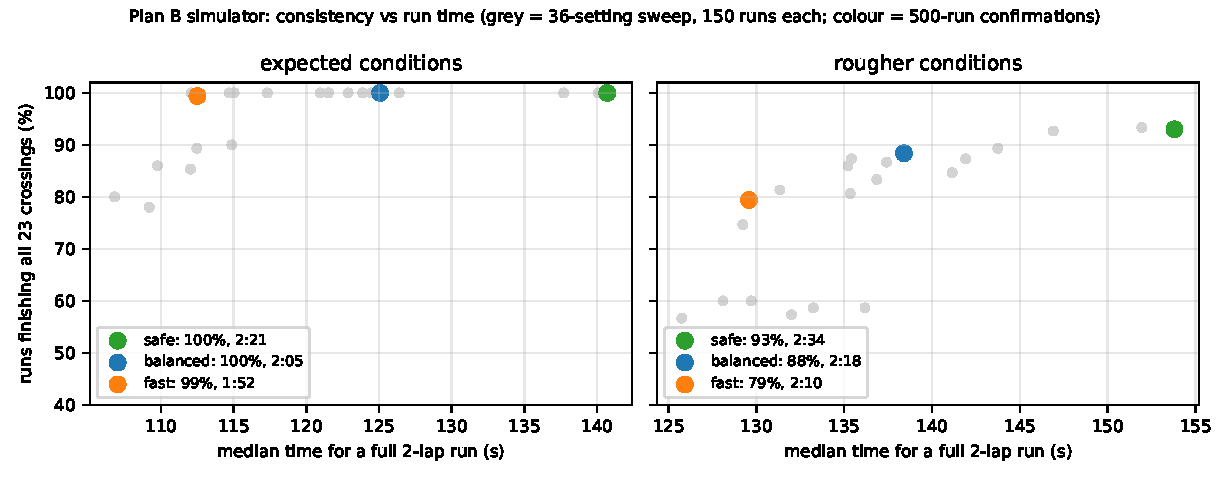
\includegraphics[width=\linewidth]{figs/planb_tradeoff.pdf}
\caption{Consistency against run time for every swept Plan B setting.}\label{fig:planbtrade}
\end{figure}

\begin{table}[H]\centering\footnotesize
\begin{tabular}{@{}lrr@{}}
\toprule
Assumption changed (setting ``balanced'', 300 runs each) & finish, expected & finish, rougher \\
\midrule
as designed & 100.0\,\% & 87.3\,\% \\
no barometer (vision height only) & 100.0\,\% & 82.7\,\% \\
detector range 8\,m & 100.0\,\% & 85.7\,\% \\
detector range 5\,m & 97.0\,\% & 47.0\,\% \\
no back-of-gate detection & 97.7\,\% & 64.3\,\% \\
gate fixes at 10\,Hz, +100\,ms latency & 99.7\,\% & 69.0\,\% \\
camera tilt unknown by 2\textdegree & 100.0\,\% & 83.0\,\% \\
camera tilt unknown by 5\textdegree & 92.3\,\% & 47.0\,\% \\
all of: no baro, 8\,m, no back view, 10\,Hz, 2\textdegree & 97.7\,\% & 45.0\,\% \\
\bottomrule
\end{tabular}
\caption{How much Plan B depends on its assumptions.}\label{tab:planbassump}
\end{table}

\begin{figure}[H]\centering
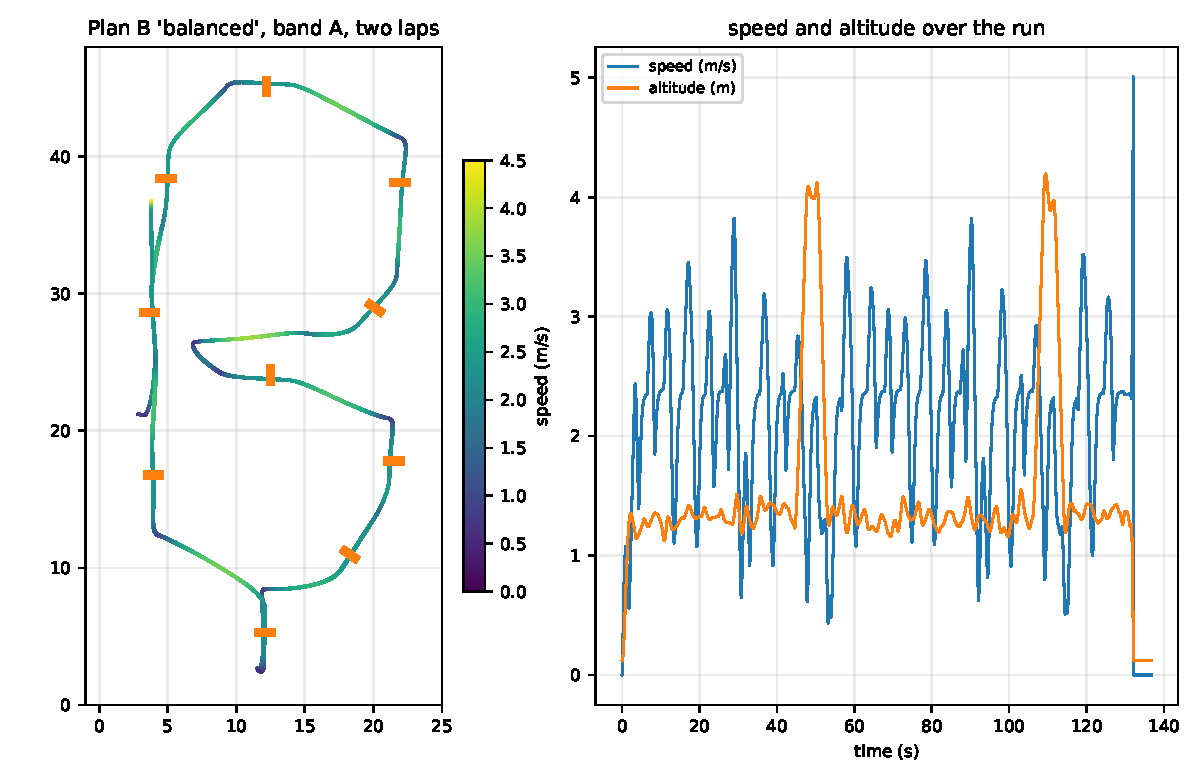
\includegraphics[width=0.95\linewidth]{figs/planb_path.pdf}
\caption{One simulated ``balanced'' run under expected conditions: split-S bypass around G6, climb to the upper opening of G9, two laps.}
\end{figure}

\begin{verdict}[Plan B verdict]
\begin{itemize}
\item \textbf{Recommended setting:} \textbf{``balanced''}. It finishes 100\,\% of runs under expected conditions and 88\,\% under rougher ones, in about \textbf{2:05} for two laps.
\item \textbf{If on-site conditions look rough:} use \textbf{``safe''} (2:21, 93\,\% under rougher conditions).
\item \textbf{Only after clean real runs:} try ``fast'' (1:52, 79\,\% under rougher conditions).
\item \textbf{Robustness under expected conditions:} it still finishes 98\,\% of runs with \emph{all} pessimistic assumptions at once.
\item \textbf{A barometer is optional.} Vision height relative to each gate teaches the thrust bias.
\item \textbf{The biggest single risk is camera tilt.} A \SI{5}{\degree} unknown tilt error drops finishing to 92\,\% (expected conditions) and 47\,\% (rougher). \textbf{Measure the tilt.}
\item \textbf{Under rough conditions,} a short detector range (5\,m), no back-of-gate detection and slow vision matter most.
\item \textbf{What limits run time:} the two forced turnarounds and the alignment pauses, not the cruise speed.
\end{itemize}
\end{verdict}

\begin{warnbox}[What this simulation does not cover]
\begin{itemize}
\item Real rotor aerodynamics near frames, and ground effect.
\item Detector false positives (orange pylons, red signage).
\item Wrong gate identity.
\item A real gate detector's accuracy. The test assumes a gate-relative pose with a few pixels of error.
\item Whether ANGLE mode is permitted; ask the organizers.
\item The airframe span; measure the real drone.
\end{itemize}
It shows that the Plan B \emph{logic and speed budget} are sound. It does not replace testing in the cage.
\end{warnbox}
